%The Large Language Models (LLMs) has shown great potential in addressing complex tasks such as mathematical reasoning, logical reasoning 

%%% start with knowledge graphs + RAG to reduce LLM hallucination
Retrieval-Augmented Generation (RAG) \cite{lewis2020retrieval} has emerged as a promising framework to reduce the hallucination of Large Language Models (LLMs) by mitigating the gap between model knowledge and factual knowledge \cite{kaddour2023challenges,zhang2023siren,huang2025survey}.
Traditional RAG usually employs an unstructured vector-indexed database as the external knowledge source, where the text corpus is indexed using pretrained encoders to support retrieval.
Recent work has explored knowledge graphs (KGs) \cite{sunthink} as a structural alternative to the external knowledge source of RAG \cite{pan2024unifying}.
KGs enjoy several advantages over the vector-indexed database in traditional RAG, 
such as representing relational information with graph structures \cite{zhang2024knowgpt}, 
integrating knowledge from heterogeneous resources \cite{pan2024unifying},
and enhancing interpretability by neural-symbolic reasoning \cite{zhang2021neural}.
Thus, KG-based RAG has demonstrated great potential in enhancing LLMs in many domains, including medical diagnosis \cite{suknowledge}, biochemistry \cite{yang2025multi}, and physics \cite{wan2025deepresearch}.

Recent KG-based RAG methods employ two approaches to retrieve information from KGs when receiving an input query \cite{luoreasoning,han2025rag,luo2025gfm}.
Retrieval-based approaches \cite{he2024g,liretrieval,yasunaga2021qa} leverage pretrained language models \cite{reimers2019sentence} to encode KG text into embeddings, and use retriever models \cite{kipf2017semi} to identify relational triplets or subgraphs in KGs that most support the query.
And agent-based methods treat LLMs as searching agents to navigate across KGs and retrieve a relational path with supporting information for a given query \cite{sunthink,luoreasoning,ma2024think}.

While KG-based RAG methods show promise in retrieving structural information for simple relational queries, their effectiveness is limited in more complex ones.
As shown in Figure~\ref{figure:illustration}, structural information in KGs alone is often sufficient for many relational queries.
For example, retrieving the relation triplet $(Alice, \textit{daughter}, Bob)$ adequately answers the question "Who is the father of Alice?".
\begin{wrapfigure}{r}{9.5cm}
\vspace{-0.3cm}
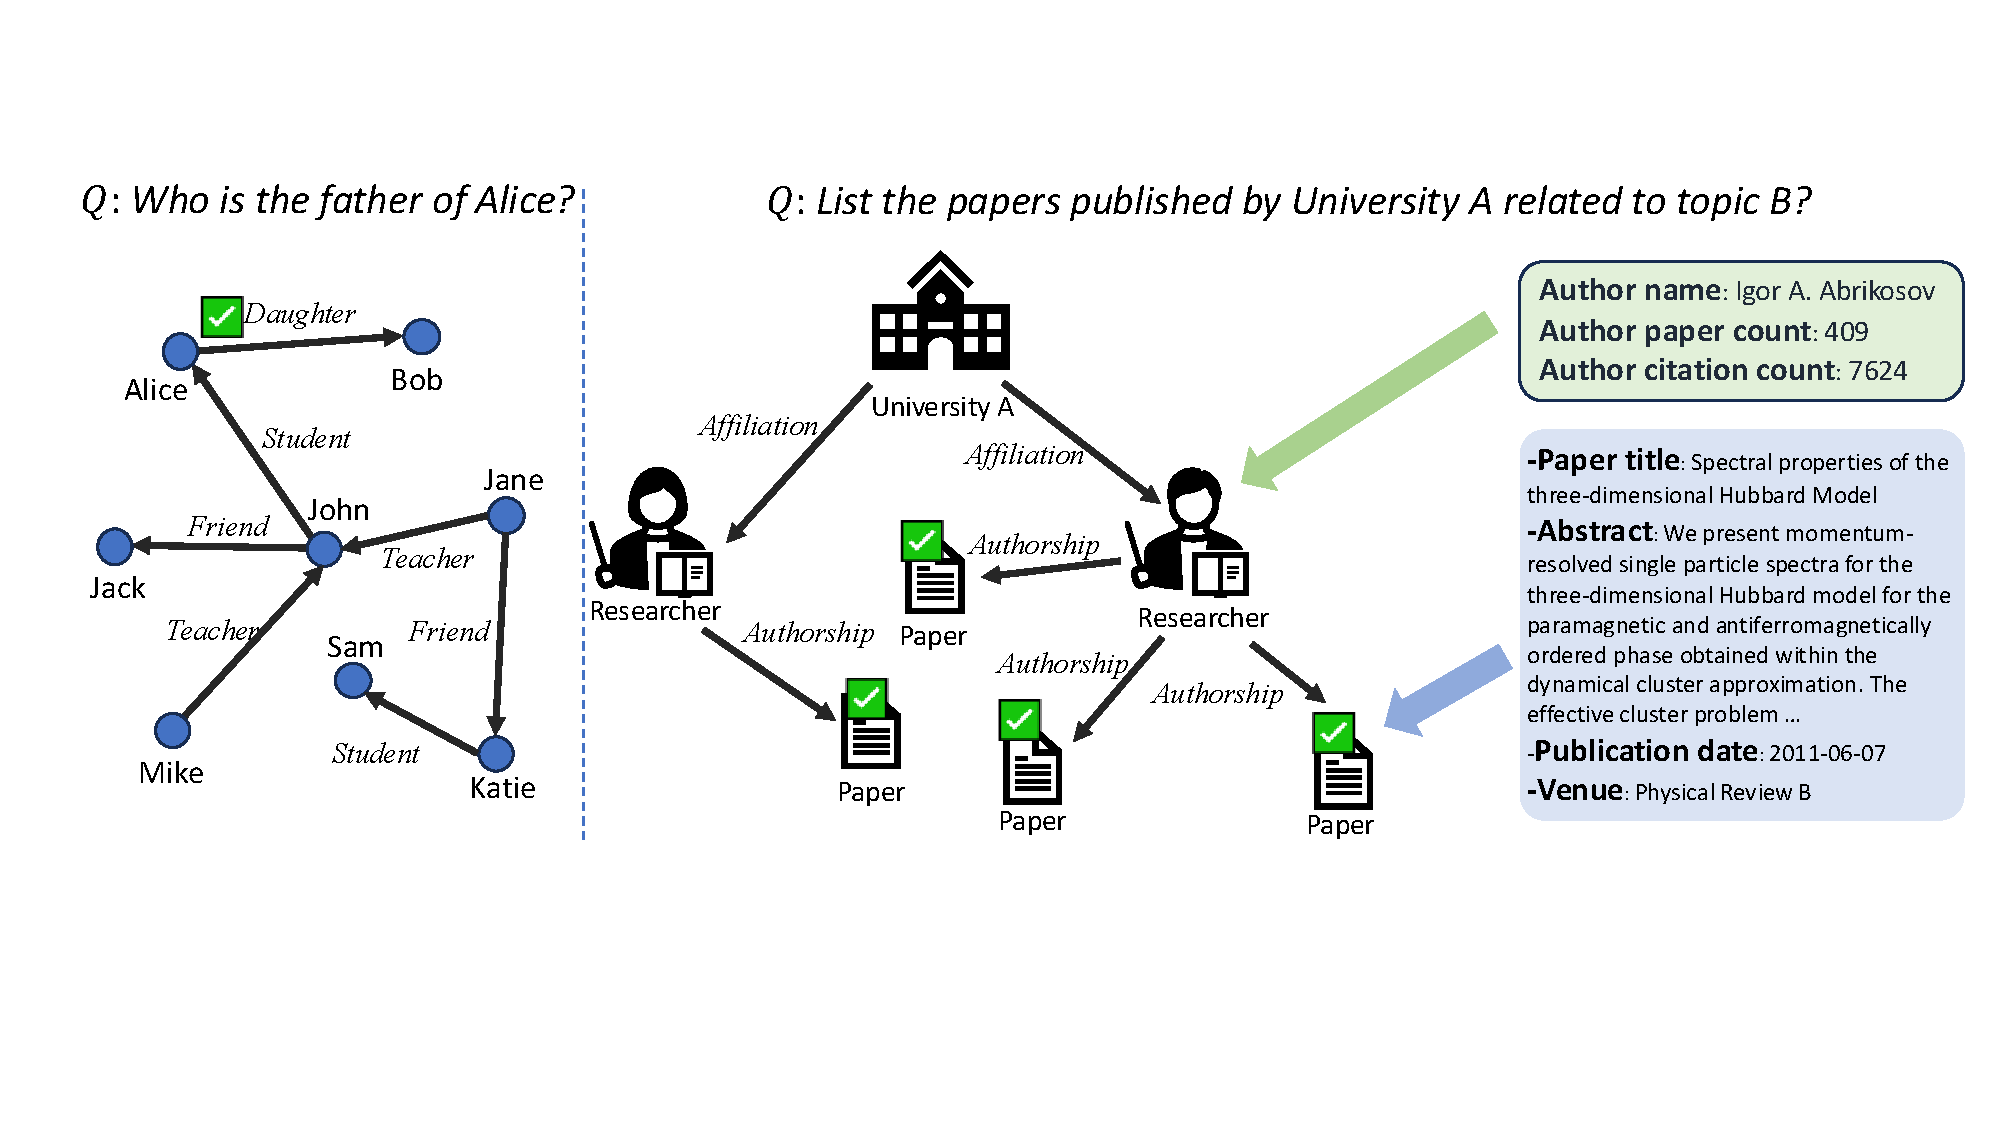
\includegraphics[width=1.0\linewidth]{newnew_illustration.pdf}
\vspace{-0.6cm}
\caption{Comparison of the retrieval tasks between relational and complex queries.} 
\vspace{-0.5cm}
\label{figure:illustration}
\end{wrapfigure}
However, complex queries typically require leveraging both structural and textual information during retrieval \cite{ma2024think}.
Consider the paper searching query "Please list the papers published by University A relevant to research topic B".
Addressing such a query requires understanding authorship and affiliation relationships, as well as text descriptions of paper content, research topics, institutions, and authors.
The fusion of relational and text knowledge presents a significant challenge for accurate retrieval with KG-based RAG methods.
Another challenge is the diversity of retrieval targets in complex queries.
Unlike relational queries corresponding to a single deterministic retrieval target (e.g., $Alice \xrightarrow{daughter} Bob$), complex queries require retrieving a diverse set of candidates.
For example, the paper searching query in Figure~\ref {figure:illustration} corresponds to multiple retrieval targets.
Therefore, KG-based RAG must emphasize both retrieval accuracy and diversity when supporting complex queries.
Unfortunately, our empirical findings reveal that existing KG-based RAG methods face challenges in achieving this goal.


To overcome the above challenge, it is essential to align the retrieval process of KG-based RAG with the diversity and accuracy demands for complex queries.
Process Reward Models (PRMs) \cite{ meng2024simpo,zhang2025lessons, zhu2025retrieval,zeng2025versaprm} offer a promising framework for this goal. 
By providing step-wise guidance, PRMs have been widely used in LLM alignment \cite{lightman2023let}, reasoning \cite{cui2025process} and planning \cite{choudhury2025process} when treating these tasks as the multi-step decision.
In KG-based RAG, the retrieval process can be naturally viewed as a multi-step decision process, where an agent traverses a KG and expands its retrieval trajectory at each step.
PRMs can provide step-wise guidance for the agent to retrieve desired information for complex queries.
However, training a PRM needs high-quality preference datasets with fine-grained and process-level reward signals \cite{nguyen2024reward, xiong2025rag, jin2025search}. 
In KG-based RAG, assessing the process-level reward at each step in retrieval trajectories is expensive.
Only the outcome reward is easily available (i.e., whether the retrieval trajectory can support a query or not).


\xhdr{Proposed Work}
We present GraphFlow, a novel framework for supporting complex queries by retrieving accurate and diverse knowledge from knowledge graphs (KGs), without relying on process-level reward supervision.
Inspired by GFlowNet \cite{bengio2023gflownet}, GraphFlow formulates the problem of retrieving from KGs as learning a retrieval policy that generates retrieval trajectories with probabilities proportional to their outcome rewards.
Thus, the retrieval trajectory that better supports the query is retrieved with a higher probability, leading to diverse and accurate retrieval results.
To achieve this, GraphFlow jointly trains the retrieval policy with a flow estimator, which assigns non-negative flow values to partial trajectories.
These flow values decompose the final outcome reward across intermediate retrieval steps, thereby providing rich supervision signals without requiring explicit process-level rewards.
The retrieval policy is guided by these flow values and receives process-level supervision “for free”.
We adopt the detailed balance objective \cite{shen2023towards} to co-train the retrieval policy and the flow estimator.
To further enhance training efficiency, we introduce a local exploration strategy that reduces visits to low-reward regions of the KG.
Thus, GraphFlow effectively explores high-reward regions of the retrieval space, leading to more accurate and diverse retrievals that better support complex query.


We evaluate the effectiveness of GraphFlow on the STaRK benchmark \cite{wu2024stark}, which involves retrieving from text-rich KGs for real-world queries across multiple domains. 
Extensive experiments demonstrate that GraphFlow consistently produces high-quality and diverse retrieval results, outperforming both Process Reward Models (PRMs) and existing KG-based RAG methods. 
Notably, GraphFlow surpasses strong KG-based RAG baselines instantiated with GPT-4o, achieving an average improvement of 10\% in both retrieval accuracy and diversity metrics. 
In addition, GraphFlow enjoys strong generalization capabilities and can retrieve from unseen KGs to support queries in new domains.



